\qns{Good Rovibrations}

\begin{enumerate}
\qitem{
	Assume we end in $n=0$.}
\work{
	\begin{align*}
		k_\text{center} &= \frac{\nu_\text{center}}{c}\\
		\nu_\text{center} &= ck_\text{center}\\
			&\approx 3(10^{10})\cdot 2145\\
			&\approx 6.4(10^{13}) \si{\hertz}\\
			&\approx 1\times\nu_{0,\text{CO}}
	\end{align*}
	where $\nu_{0,\text{CO}} \approx 6.7(10^{13}) \si{\hertz}$ is the natural frequency of CO's vibrational transition.}
\ans{
	\centering
	$|\Delta n| = 1$}

\qitem{
	\begin{itemize}
		\item Boltzmann statistics for populations in each $J$ state
		\item Line intensity $\propto$ $n_{J_\text{upper}}$
	\end{itemize}}
\work{
	\begin{align*}
	    \frac{n_{J+1}}{n_J} &= \frac{g_{J+1}}{g_J}e^{-\frac{E_{J+1} - E_J}{k_BT}}\\
			\text{where } E_{J+1} - E_J &= \frac{\hbar^2}{2I}\left[(J+1)(J+2) - J(J+1)\right]\\
			&= \frac{\hbar^2}{I}(J+1) % \longleftarrow \begin{cases}
				% I \approx \mu x_0^2\\
				% \mu \equiv m_O \parallel m_C\\
				% x_0 \approx 2.4a_0
				% 	\end{cases}\\
	\end{align*}
	Sweeping $\frac{n_{J+1}}{n_J}$ with respect to $T$ and choosing $J_\text{infl}=7$ where $\frac{n_{J_\text{infl}}}{n_{J_\text{infl}-1}} > 1$ and $\frac{n_{J_\text{infl}+1}}{n_{J_\text{infl}}} < 1$ yields a rough temperature range $T\in[288, 365)\si{\kelvin}$
	\begin{figure}[H]
		\centering
		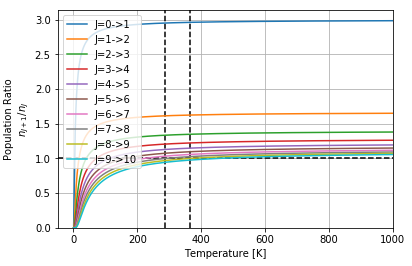
\includegraphics[width=0.48\textwidth]{./questions/q_good_rovibrations_figs/ans_pop_ratio.png}
		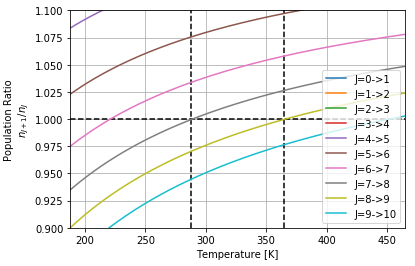
\includegraphics[width=0.48\textwidth]{./questions/q_good_rovibrations_figs/ans_pop_ratio_zoomed.png}
		\caption{The population ratios vs. temperature for different values of $J\rightarrow J+1$}
		\label{fig:ratio_vs_temp}
	\end{figure}}
\ans{
	\centering
	Because $n_{J=6} \approx n_{J=7}$
	$$T \approx 288\si{\kelvin}$$
}

\qitem{}
\work{
	Looking up the dipole moment $d_\text{CO} \approx 0.122 \text{ esu.}\si{\centi\meter}$ and calculating values relative to the Lyman-$\alpha$
	$$A_\text{CO} =  A_{\text{Ly}\alpha}\left(\frac{d_\text{CO}}{d_\text{H}}\right)^2\left(\frac{\omega_\text{CO}}{\omega_{\text{Ly}\alpha}}\right)^3$$
	with
	\begin{align}
		\omega_\text{CO} &= \frac{(\Delta E)_{\substack{\Delta n=1\\\Delta J=\pm1}}}{\hbar}\\
			&= \omega_{0,\text{CO}} \pm \frac{\hbar}{I}J_\text{upper} \label{eqn:Iconst}
	\end{align}
	Eqn. \ref{eqn:Iconst} assumes a constant moment of inertia.
	In reality, there will be a change in interatomic distance dependent on $n$, i.e. the moment of inertia will increase with $n$.
	\begin{figure}[H]
		\centering
		\begin{subfigure}[t]{0.48\linewidth}
			\centering
			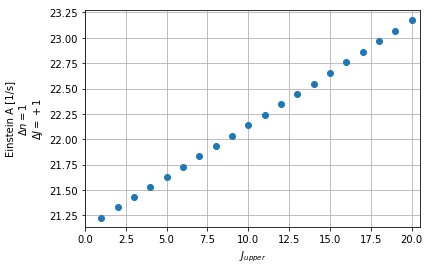
\includegraphics[width=\textwidth]{./questions/q_good_rovibrations_figs/ans_A_dJp1.png}
			\caption{}
			\label{subfig:A_vs_J_plus1}
		\end{subfigure}
		\begin{subfigure}[t]{0.48\linewidth}
			\centering
			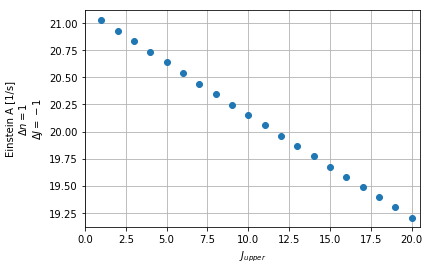
\includegraphics[width=\textwidth]{./questions/q_good_rovibrations_figs/ans_A_dJm1.png}
			\caption{}
			\label{subfig:A_vs_J_minus1}
		\end{subfigure}
		\label{fig:A_vs_J}
		\caption{Calculated Einstein A coefficients for the R (\subref{subfig:A_vs_J_plus1}) and P (\subref{subfig:A_vs_J_minus1}) branches}
	\end{figure}}
\ans{
	\centering
	$A$ varies by more than 10\% over the range of $J$---probably enough to warrant inclusion.}

\qitem{}
\work{
	\begin{align*}
		j_\nu &= \frac{h\nu}{4\pi}n_{J_\text{upper}}A_{21}\phi(\nu)
	\end{align*}
	Supposing $\phi(\nu)$ is constant across frequency,}
\ans{
	\begin{figure}[H]
		\centering
		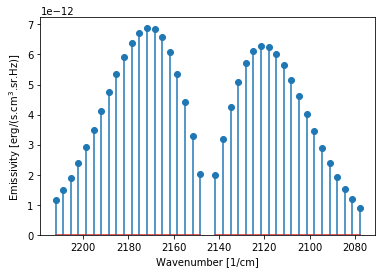
\includegraphics[scale=0.8]{./questions/q_good_rovibrations_figs/ans_emissivity_cheating.png}
		\label{fig:emissivity}
		\caption{Emissivity assuming $\nu_0 = 2145\si{\centi\meter^{-1}}\cdot c$.}
	\end{figure}}

\qitem{\textcolor{white}{blep}}
\ans{
	Some final discrepancies:
	\begin{itemize}
		\item non-constant line profile function vs. frequency (i.e. Heisenberg uncertainty and Doppler spread) would have each peak smeared out across frequencies 
		\item change in the interatomic distance and consequently the moment of inertia with respect to vibrational energy would cause spreading between the peaks of the P branch vs. the R branch
	\end{itemize}}
\end{enumerate}